% !TeX encoding = UTF-8
% !TeX spellcheck = en_US
% !TEX root = midterm_exam_WS2324.tex
\documentclass{article}
%%%%%%%%%%%%%%%%%%%%%%%%%%%%%%%%%%%%%%%%%%%%%%%%%%%%%%%%%%%%%%%%%%%%%%%%%%%%%%%%%%%%%%%%%%%%%%%%%%%%%%%%%%%%%%%%%%%%%%%%%%%%%%%%%%%%%%%%%%%%%%%%%%%%%%%%%%%%%%%%%%%%%%%%%%%%%%%%%%%%%%%%%%%%%%%%%%%%%%%%%%%%%%%%%%%%%%%%%%%%%%%%%%%%%%%%%%%%%%%%%%%%%%%%%%%%
\usepackage[a4paper,top=2cm]{geometry}
\usepackage{amssymb,amsmath,amsfonts}
\usepackage[english]{babel}
\usepackage[a4paper]{geometry}
\usepackage{enumitem}
\usepackage{booktabs}
\usepackage{csquotes}
\usepackage{graphicx}
\usepackage[numbered,framed]{matlab-prettifier}
\usepackage{url}
%\parindent0mm
%\parskip1.5ex plus0.5ex minus0.5ex
\usepackage[backend=biber,style=authoryear]{biblatex}
\addbibresource{../literature/_biblio.bib}
\begin{document}
	
\title{Quantitative Macroeconomics}
\author{Midterm Exam}
\date{Winter 2023/2024}
\maketitle

\section*{General information}
\begin{itemize}
	\item Answer \textbf{all} of the following \textbf{four} exercises in English.
	\item All assignments will be given the same weight in the final grade.
	\item Hand in your solutions before January, 10 2024 at 3pm.
	\item The solution files should contain your executable (and commented) script files
		as well as all additional documentation as \texttt{pdf}, not \texttt{txt}, \texttt{md}, \texttt{tex}, \texttt{doc} or \texttt{docx}.
	Your \texttt{pdf} files may also include scans or pictures of handwritten notes.
	\item Please e-mail ALL the solution files to \url{willi.mutschler@uni-tuebingen.de}.
	I will confirm the receipt of your work also by email (typically within the hour). If not, please resend it to me.
	\item All students must work on their own, please also give your student ID number and the name of the module you want to earn credits for.
	\item It is advised to regularly check Ilias and your emails in case of urgent updates.
	\item If there are any questions, do not hesitate to contact Willi Mutschler.
\end{itemize}

\newpage

	
\section[Theoretical and Simulated Moments]{Theoretical and Simulated Moments\label{ex:TheoreticalAndSimulatedMoments}}
\begin{enumerate}
 	\item Derive the unconditional first two moments (i.e.\ theoretical mean, covariance and autocovariance matrix) of the covariance stationary VAR(1) model: \(y_t = \nu + A y_{t-1} + u_t\)
 	\item Simulate \(R=100\) datasets each with \(T=100\) observations for
 	\begin{align*}
 	y_t = \begin{pmatrix}0.2 &0.3 \\-0.6 & 1.1 \end{pmatrix} y_{t-1}  + u_t
 	\end{align*}
 	provided that \(u_t \sim WN(0,\Sigma_u)\) and \(\Sigma_u = \begin{pmatrix}0.9 &  \\ 0.2 & 0.5 \end{pmatrix}\).
	\item Compute the sample mean and sample covariance matrix for each of the \(R\) datasets. 
	Then take the average and compare the results with part (1).
	\item How does your choice of \(R\) or \(T\) change your results?
	
\end{enumerate}

\newpage


\section{Properties Of Lag-Order Selection Criteria}
Assume that the true Data-Generating-Process (DGP) follows the following VAR(4) model
\begin{align*}
y_t = \begin{pmatrix}
2.4 & 1.0\\
0 & 1.1
\end{pmatrix}
y_{t-1}+
\begin{pmatrix}
-2.15 & -0.9\\
0 & -0.41
\end{pmatrix}
y_{t-2}+
\begin{pmatrix}
0.852 & 0.2\\
0& 0.06
\end{pmatrix}
y_{t-3}+
\begin{pmatrix}
-0.126 & 0\\
0 & 0.0003
\end{pmatrix}
y_{t-4}
+ u_t
\end{align*}
where \(u_t\) is a Gaussian white noise with contemporary covariance matrix \(\Sigma_u = \begin{pmatrix}
0.9&0.2\\0.2&0.5
\end{pmatrix}\).

Perform a Monte-Carlo analysis to study both the finite-sample as well as asymptotic properties
of the Akaike Information Criterion (AIC) and the Schwarz Information Criterion (SIC):
\begin{align*}
AIC(m)  &= \log(det(\tilde{\Sigma}_u(m))) + \frac{2}{T}\varphi(m)\\
SIC(m)  &= \log(det(\tilde{\Sigma}_u(m))) + \frac{\log T}{T}\varphi(m)
\end{align*}
where \(\tilde{\Sigma}_u=T^{-1}\sum_{t=1}^T \hat{u}_t\hat{u}_t'\) is the residual covariance matrix estimator
for a reduced-form VAR model of order $m$ based on OLS residuals \(\hat{u}_t\).
The function \(\varphi(m)\) corresponds to the total number of regressors in the system of VAR equations.
The VAR order is chosen such that the respective criterion is minimized over the possible orders \(m = 0,\ldots,p^{max}\).
To this end, do the following.

\begin{itemize}
	\item Set the number of Monte Carlo repetitions \(R=100\) and \(p^{max}=8\).
	\item Initialize output matrices \(aic\) and \(sic\) each of dimension \(R \times 5\).
	\item For \(r=1,\ldots,R\) do the following:
	\begin{itemize}
		\item Simulate \(10100\) observations for the DGP given above and discard the first 100 observations as burn-in phase.
		Save the remaining 10000 observations in a matrix \(Y\).
		\item Compute the lag criteria for 5 different sample sizes \(T=\{80, 160, 240, 500, 10000\} \),
		i.e.\ use the last \(T\) observations of your simulated data matrix \(Y\) for computations.
		\item Save the chosen lag order in the corresponding output object at position \([r,j]\) where \(j=1,\ldots,5\) indicates the corresponding sample size.
	\end{itemize}
	\item Look at the frequency tables of your output objects for the different subsamples. Hint: \texttt{tabulate(aic(:,1))} displays a frequency table for the AIC criterion with sample size equal to 80.
\end{itemize}
Given your results, do you agree with the following (general) findings?
\begin{enumerate}
	\item AIC is not consistent for the true lag order, whereas SIC is consistent.
	\item AIC never (asymptotically) selects a lag order that is lower than the true lag order.
	\item In finite samples, we usually have \(\hat{p}_{SIC} \leq \hat{p}_{AIC}\).
	\item In finite samples, AIC has a tendency to overestimate the lag order, SIC has a tendency to underestimate the lag order; hence, one should rely on AIC in finite samples.
\end{enumerate}

\newpage

\section[Sign-identified Monetary SVAR Model for US]{Sign-identified Monetary SVAR Model for US\label{ex:SignIdentifiedMonetarySVARUS}}
Consider data for \(y_t = (\Delta gnp_t,\Delta p_t,i_t)'\),
  where \(gnp_t\) denotes the log of U.S. real GNP,
  \(p_t\) the consumer price index in logs,
  and \(i_t\) the federal funds rate.
  Data is given in the csv file \texttt{MonPol.csv} containing the sample period of 1970Q1 to 2011Q1.

We will use the following sign restrictions pattern to identify the structural shocks:
\begin{align}
B_0^{-1}=\begin{bmatrix}
	+ & + & -\\
	+ & - & -\\
	+ & *  & +
	\label{eq:signpattern}
\end{bmatrix}
\end{align}
where \(*\) denotes an unrestricted value.

\begin{enumerate}
\item Read the short summary paper by \textcite{Wolf_2022_WhatCanWe} and provide economic intuition for the pattern given in equation \eqref{eq:signpattern}.
\item Write a script that estimates the structural impulse response function via sign restrictions.
To this end:
	\begin{itemize}
	\item Estimate a VAR(4) model with constant by using ordinary least-squares.
	Compute the lower Cholesky decomposition of your estimated residual covariance matrix, i.e.\ \( P = chol(\hat{\Sigma}_u) \).
	\item Set the IRF horizon \(H=20\) and the number of required sign-identified draws to \(N=1000\).
	\item Initialize an array \texttt{IRFvals} of dimension
	(i) number of variables \(K\) by (ii) number of shocks \(K\) by (iii) horizon \(H\) by (iv) number of draws \(N\).
	This array will store \(n=1,\ldots,N\) sign-identified impulse response functions \(\theta_{jkhn}\) for variable \(j=1,\ldots,K\)
	with respect to shock \(k=1,\ldots,K\) at horizon \(h=0,\ldots,H\), where \(K\) is the number of variables.
	
	\item Initialize \texttt{n=1} and write a while loop that executes the following steps:
		\begin{itemize}
		\item Draw an orthogonal rotation matrix \(Q\) using the function \texttt{drawRotationMatrixQ.m} in the appendix.
		\item Compute the implied rotated impact matrix \(\widetilde{B}_0^{-1}=PQ\).
		\item Note that \(\widetilde{B}_0^{-1}\) is a valid impact matrix, because \(\hat{\Sigma}_u = \widetilde{B}_0^{-1} \widetilde{B}_0^{-1'}\).
		However, we will only accept those impact matrices \(\widetilde{B}_0^{-1}\) that full-fill the sign restrictions in equation~\eqref{eq:signpattern}.
		Therefore, use if statements to check whether \(\widetilde{B}_0^{-1}\) is a valid impact matrix:
		\begin{itemize}
			\item If the pattern is correct, increase \(n\) by 1 and compute the implied IRFs. Store these into \texttt{IRFvals(:,:,:,n)}.
			\item If the pattern is incorrect, don't change the value of \(n\), discard this draw and go back to the beginning of the loop.
			\end{itemize}
		\item End the while loop if \texttt{n=N}.
		\end{itemize}
	\item Plot \textbf{ALL} \(N\) impulse response functions that full-fill the sign pattern for (i) the level of GDP, (ii) CPI inflation and (iii) the Federal Funds rate.
	\\Hint: The graphs should look similar to figure~\ref{fig:signSVAR} in the appendix.
	That is, in each subplot compute and plot \texttt{IRFS = squeeze(IRFvals(ivar,ishock,1:nsteps,:))}.	
	\end{itemize}
\end{enumerate}

\newpage

\section[Historical Decomposition]{Historical Decomposition}
Reconsider the SVAR model of \textcite{Rubio-Ramirez.Waggoner.Zha_2010_StructuralVectorAutoregressions}
(i.e. the exercise called \emph{Combining Short-Run And Long-Run Restrictions}).

A historical decomposition is a tool to quantify how important a structural shock was 
in driving the behavior of the endogenous variables in a specific time period in the past.
It allows to track at each point in time the role of structural shocks
in driving the VAR's endogenous variables away from their steady state.

Given the notation used in the lecture, the historical decomposition for a VAR(1)
is based on the following recursive Wold representation:
\begin{align*}
y_t = A^t y_0 + \sum_{j=0}^{t-1} A^j B_0^{-1} \varepsilon_{t-j}
\end{align*}
Therefore, the historical decomposition of say \(y_{2}\) is given as a function of present and past structural shocks
plus the initial condition:
\begin{align*}
y_{2} = \underbrace{A^2 y_0}_{\text{initial}} + \underbrace{A B_0^{-1}}_{\Theta_1} \varepsilon_{1} + \underbrace{B_0^{-1}}_{\Theta_0} \varepsilon_{2}
\end{align*}
Write an algorithm to compute the historical decomposition of the federal funds rate with respect to the three shocks in the model.

Hints:
\begin{itemize}
	\item Use the companion form.
\end{itemize} 

\newpage
\appendix

\printbibliography
\newpage
\section{Codes}
\lstinputlisting[label=drawRotationMatrixQ,title=\lstname,style=Matlab-editor,basicstyle=\footnotesize\mlttfamily,title=\lstname]{../progs/matlab/drawRotationMatrixQ.m}

\newpage

\section{Figures}
\begin{figure}[htbp]\caption[]{Sign-identified IRFs}\label{fig:signSVAR}
	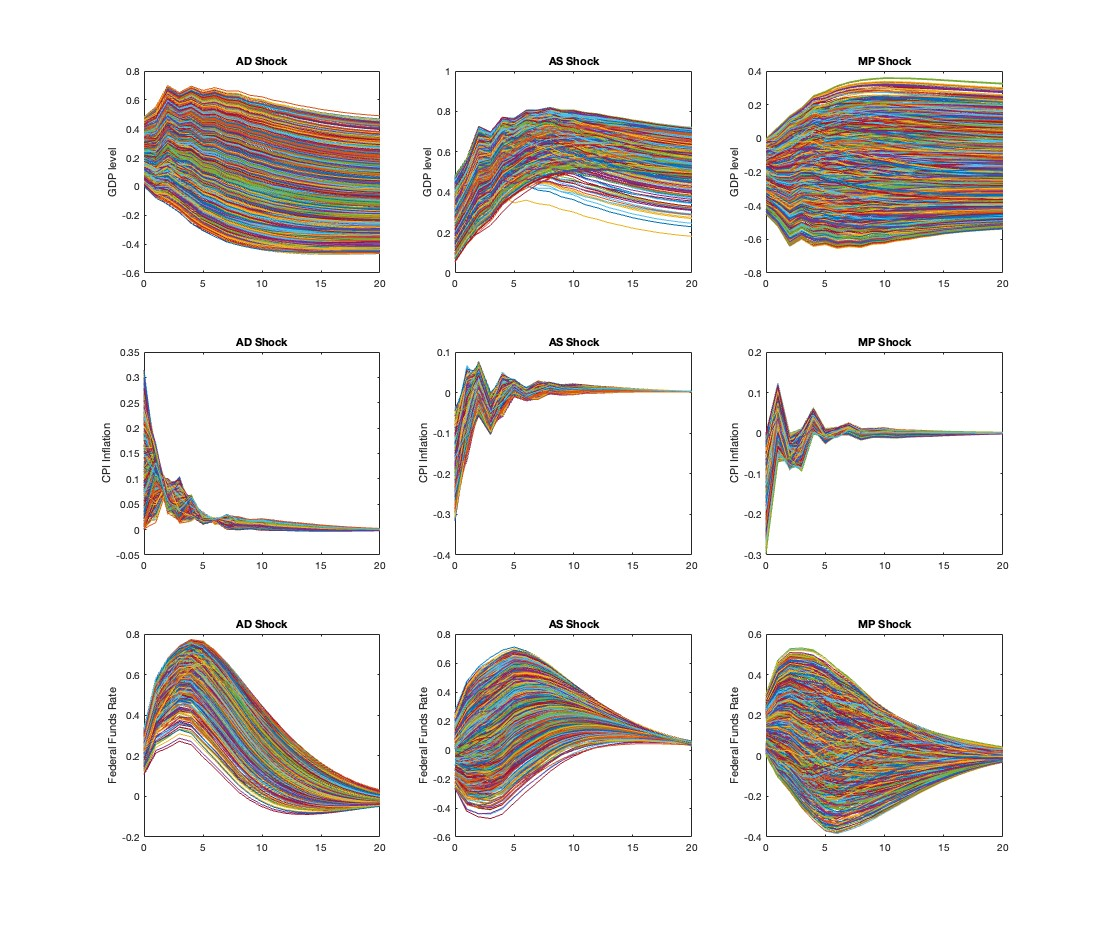
\includegraphics[width=\textwidth]{../plots/signIRFs.jpg}
\end{figure}

\end{document}